\documentclass[lualatex,aspectratio=169,xcolor=dvipsnames,10pt,c]{beamer}

%\usepackage{booktabs}
%\usepackage{setspace}
%\usepackage{framed}

% Graphics
%\usepackage{pgfpages}
%\setbeameroption{show notes on second screen=right}
%\setbeameroption{show notes}
\usepackage{graphbox} %loads graphicx package
\usepackage{multimedia}
\usepackage{tikz}
\graphicspath{{figures/}{generated-figures/}{video/}}

% Fonts and template
% see: https://github.com/ibab/beamertheme-vertex/blob/master/beamerthemevertex.sty
\usepackage{fontspec}%	
\usepackage[default]{sourcesanspro}
\usefonttheme{professionalfonts} 
\usepackage{unicode-math}
\newfontfamily\ExtraLight{Source Sans Pro Extra Light}%
\newfontfamily\LightOldStyle[Numbers=OldStyle]{Source Sans Pro Light}%
\newfontfamily\Light{Source Sans Pro Light}%
\newfontfamily\Regular{Source Sans Pro}%
\newfontfamily\Bold{Source Sans Pro Bold}%
\newfontfamily\Black{Source Sans Pro Bold}%
\setsansfont{Source Sans Pro Light}%
\setmonofont[Scale=MatchLowercase]{Source Code Pro}%
\setmathfont{Latin Modern Math}
\setbeamerfont{frametitle}{family=\LightOldStyle,size=\Large}
\setbeamerfont{section in toc}{family=\Light}
\setbeamertemplate{frametitle}{\vspace{.4cm}\insertframetitle}
\setbeamertemplate{footline}[frame number]
\setbeamertemplate{navigation symbols}{}
\setbeamercolor{alerted text}{fg=black}
\setbeamerfont{alerted text}{series=\bfseries}

\newcommand{\prescite}[1]{{\small \textcolor{gray}{#1}}}

% Specific environments
\usepackage{alltt}
\usepackage{xspace}

% Meta
\title{Localization of inexpensive robots with low-bandwidth sensors}

\author[Wang et al.]{Shiling Wang, Francis Colas, Ming Liu, Francesco Mondada, Stéphane Magnenat\\ %
	\vspace{1em} 
	\raisebox{.01\textwidth}{
\includegraphics[height=.03\textwidth]{eth_logo_kurz_pos}}\qquad
	
\includegraphics[height=.05\textwidth]{inria-logo-scientifique-uk}\qquad
	\raisebox{-.005\textwidth}{
\includegraphics[height=.06\textwidth]{cuhk-logo}}\qquad
	
\includegraphics[height=.05\textwidth]{epfl_logo}
}

\date{November 9, 2016}


\begin{document}

\section*{}

\sourcesansprolight

\frame[plain]{\titlepage}

{
	\setbeamercolor{page number in head/foot}{fg=white}
	\frame
	{
		\begin{tikzpicture}[remember picture,overlay,shift=(current page.center)]
			\node at (0,0){
				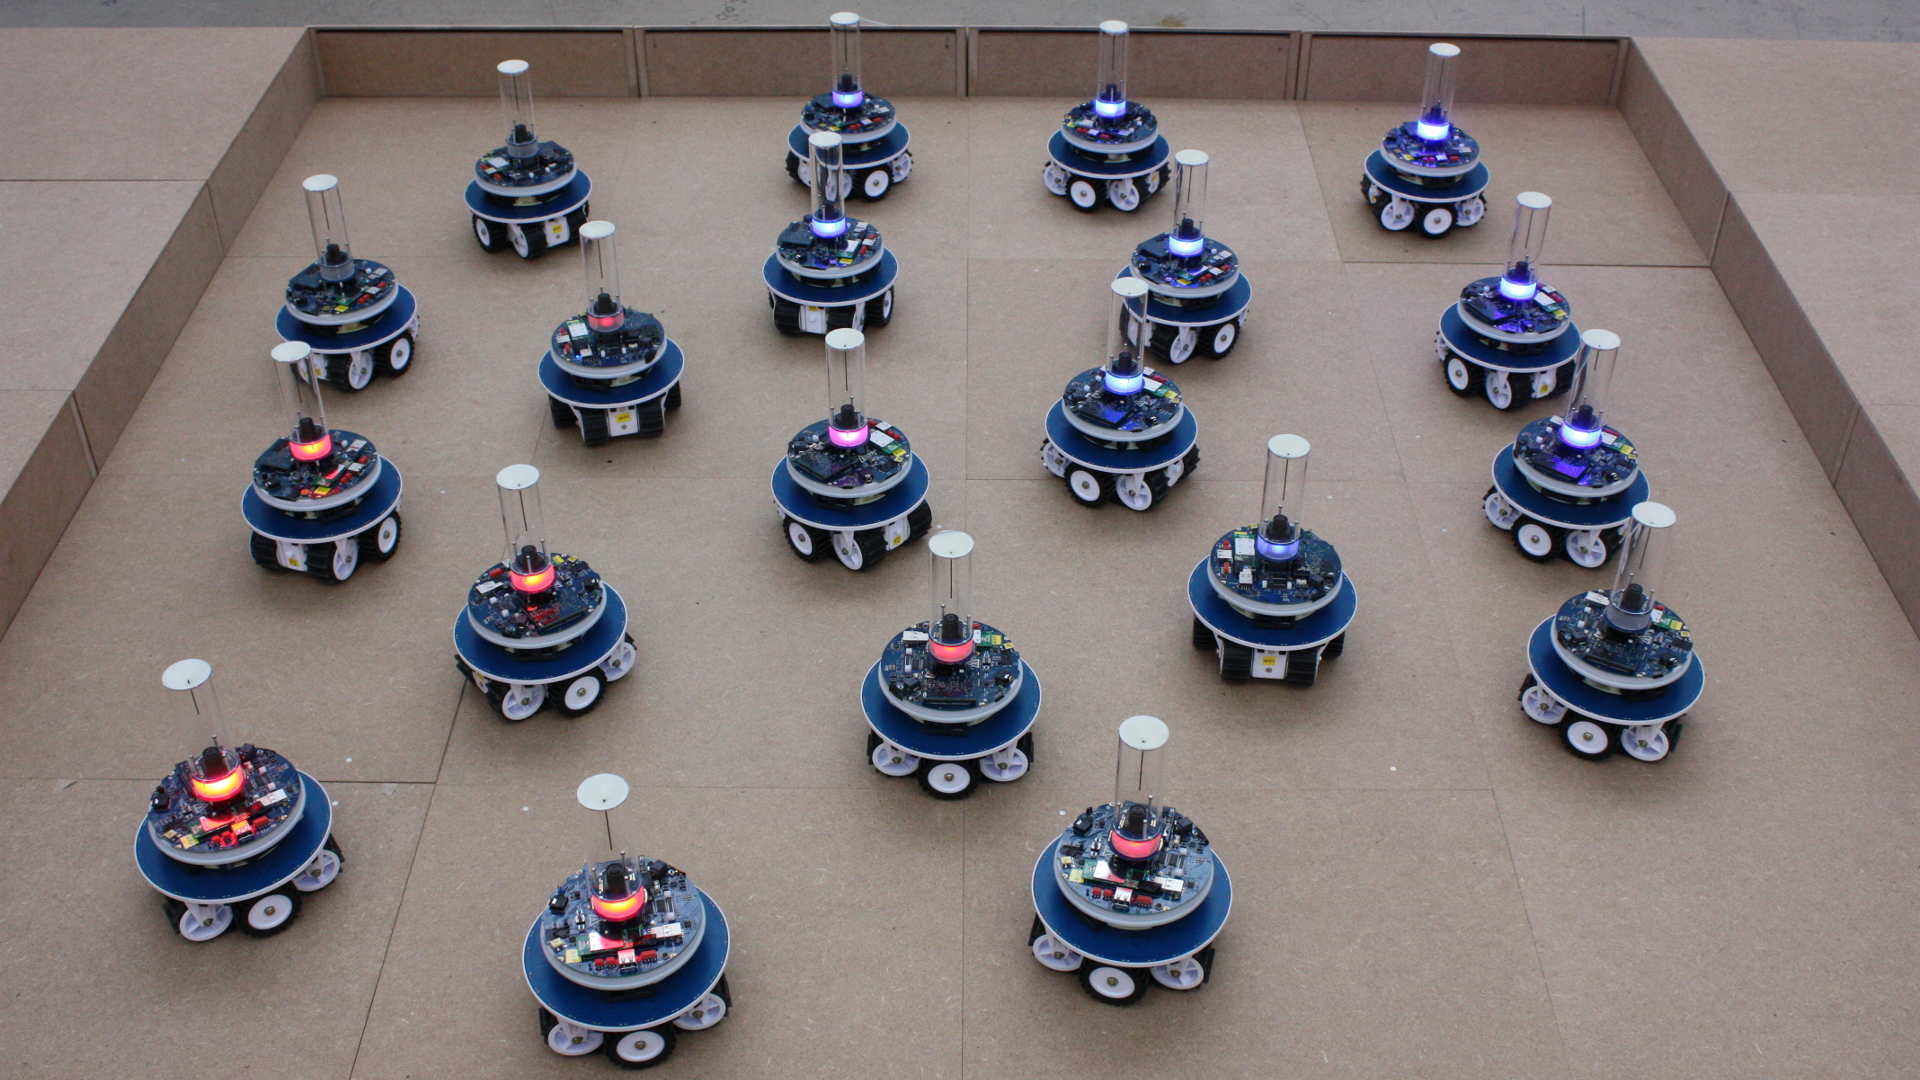
\includegraphics[width=\paperwidth]{marxbots}
			};
		\end{tikzpicture}
		
		\note{Problem: localize inexpensive mobile robots}
	}
}

\frame
{
	\frametitle{Related Work}
	
	\begin{columns}
	\column{.45\textwidth}
	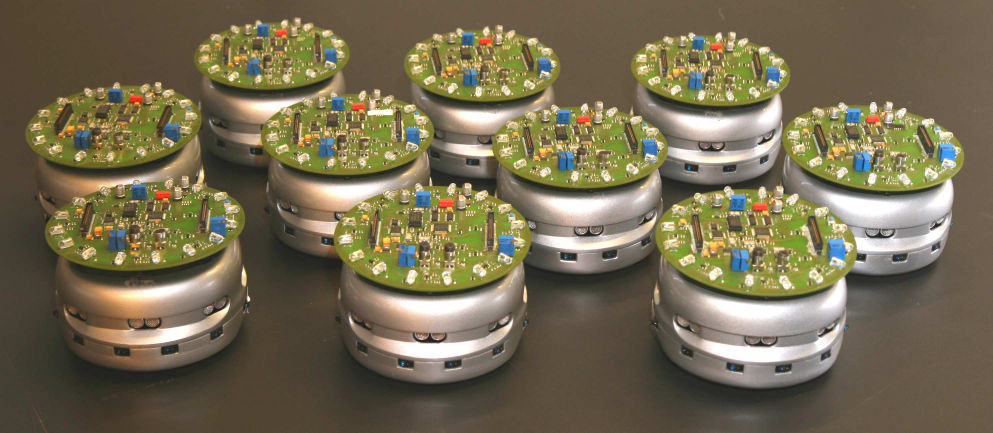
\includegraphics[width=.9\columnwidth]{prorok-robots}
	
	\footnotesize{Prorok et al., Low-cost collaborative localization for large-scale multi-robot systems}
	
	\vspace{1em}

	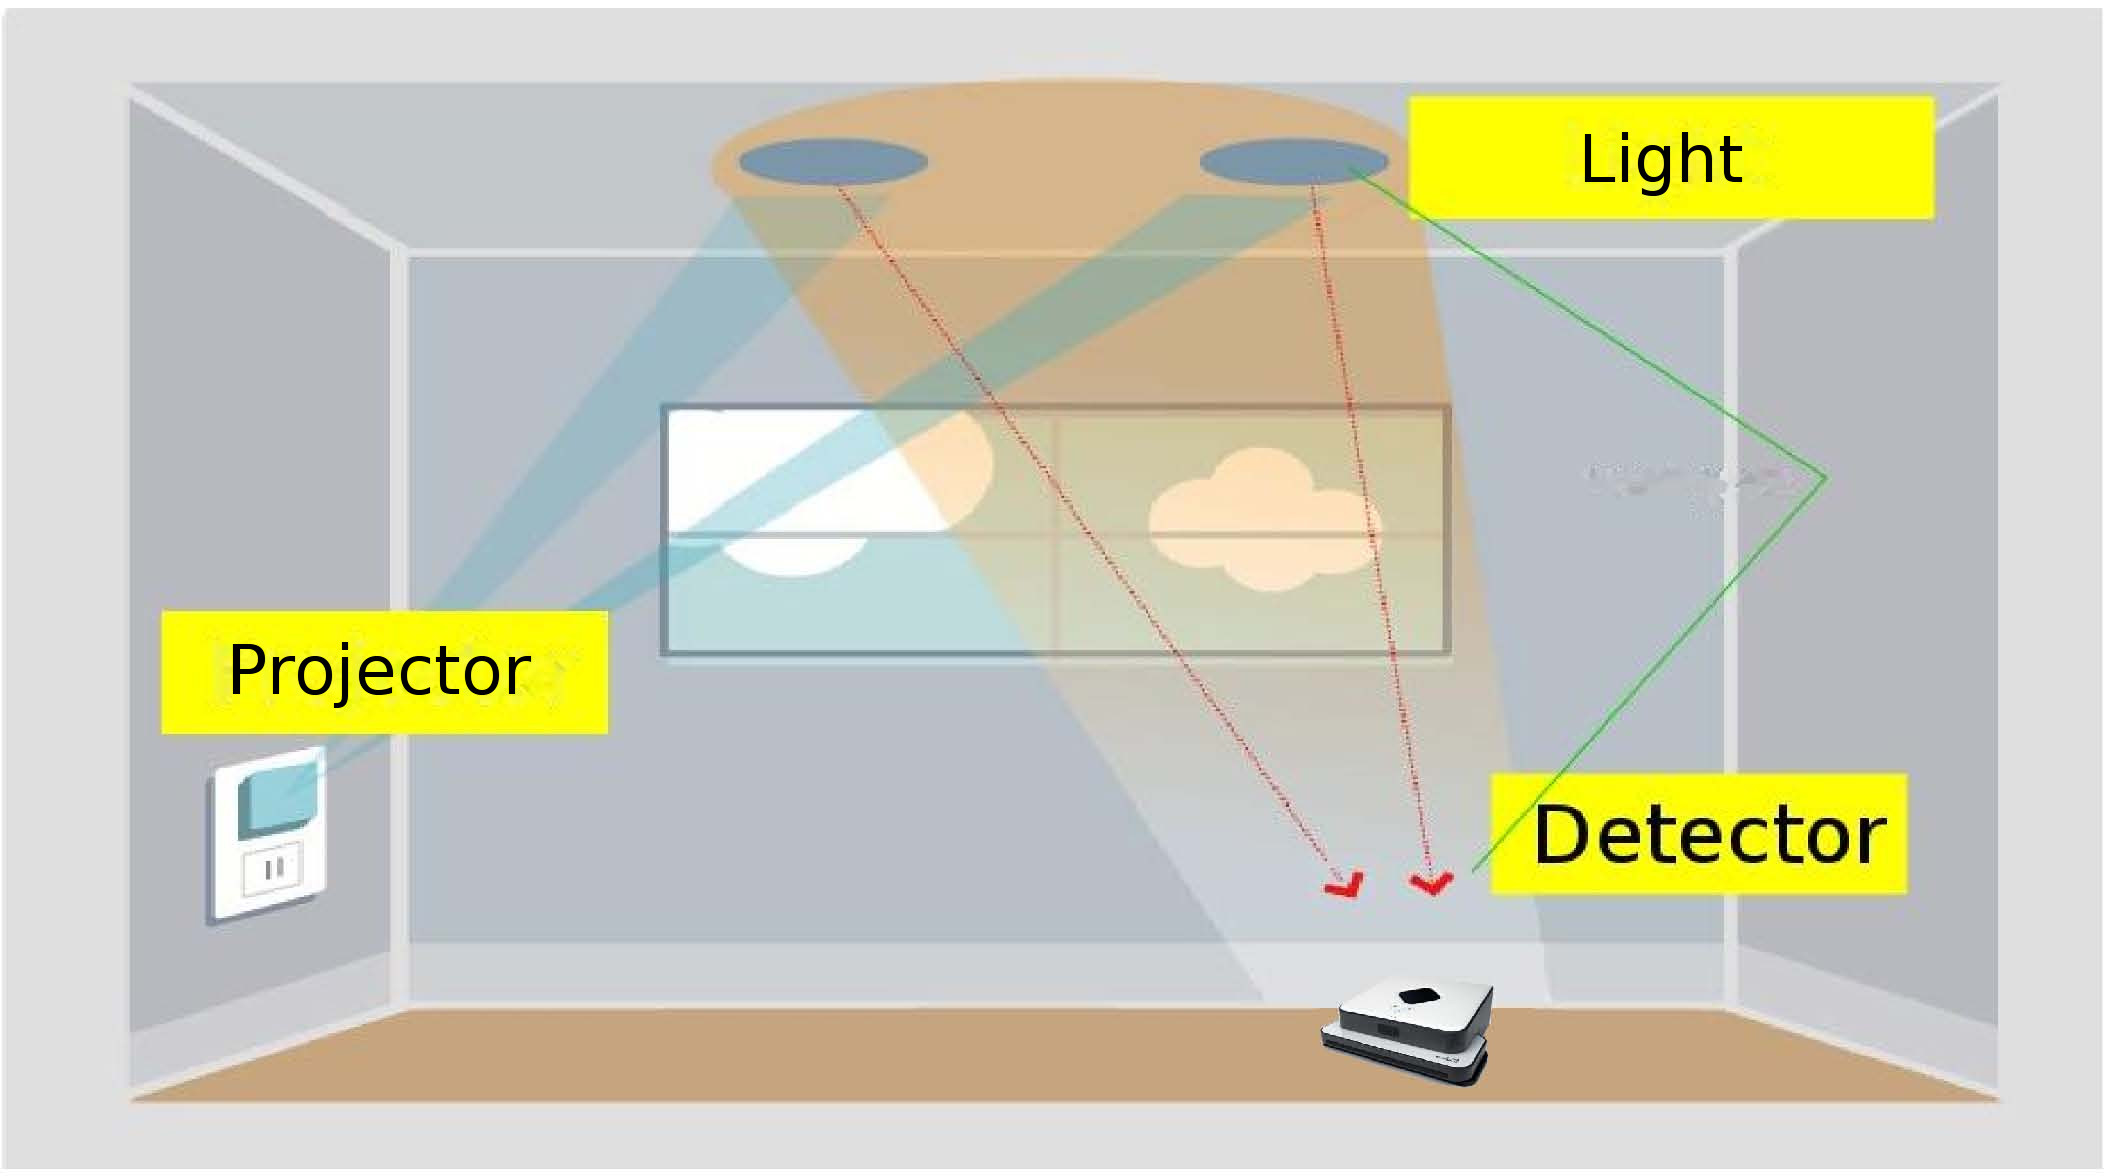
\includegraphics[width=.9\columnwidth]{gutmann-detector}
	
	\footnotesize{Gutmann et al., Challenges of designing a low-cost indoor localization system using active beacons ceiling}
	
	\column{.45\textwidth}
	
	
\includegraphics[width=.9\columnwidth]{dias-barcode}
	
	\footnotesize{Dias et al, Absolute localization for low capability robots in structured environments using barcode landmarks}
	
	\vspace{1em}
	
	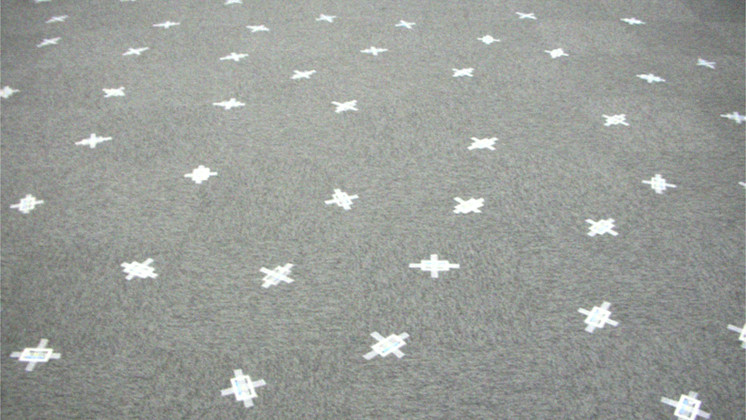
\includegraphics[width=.9\columnwidth]{park-rfid}
	
	\footnotesize{Park et al., An approach for mobile robot navigation under randomly distributed passive RFID environment}
	
	\end{columns}
}

\frame
{
	\frametitle{Our approach – Recursive Bayesian Filter}

	\raisebox{.03\columnwidth}{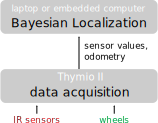
\includegraphics[width=.4\columnwidth]{system-bloc-scheme-pres}}
	\hfill
	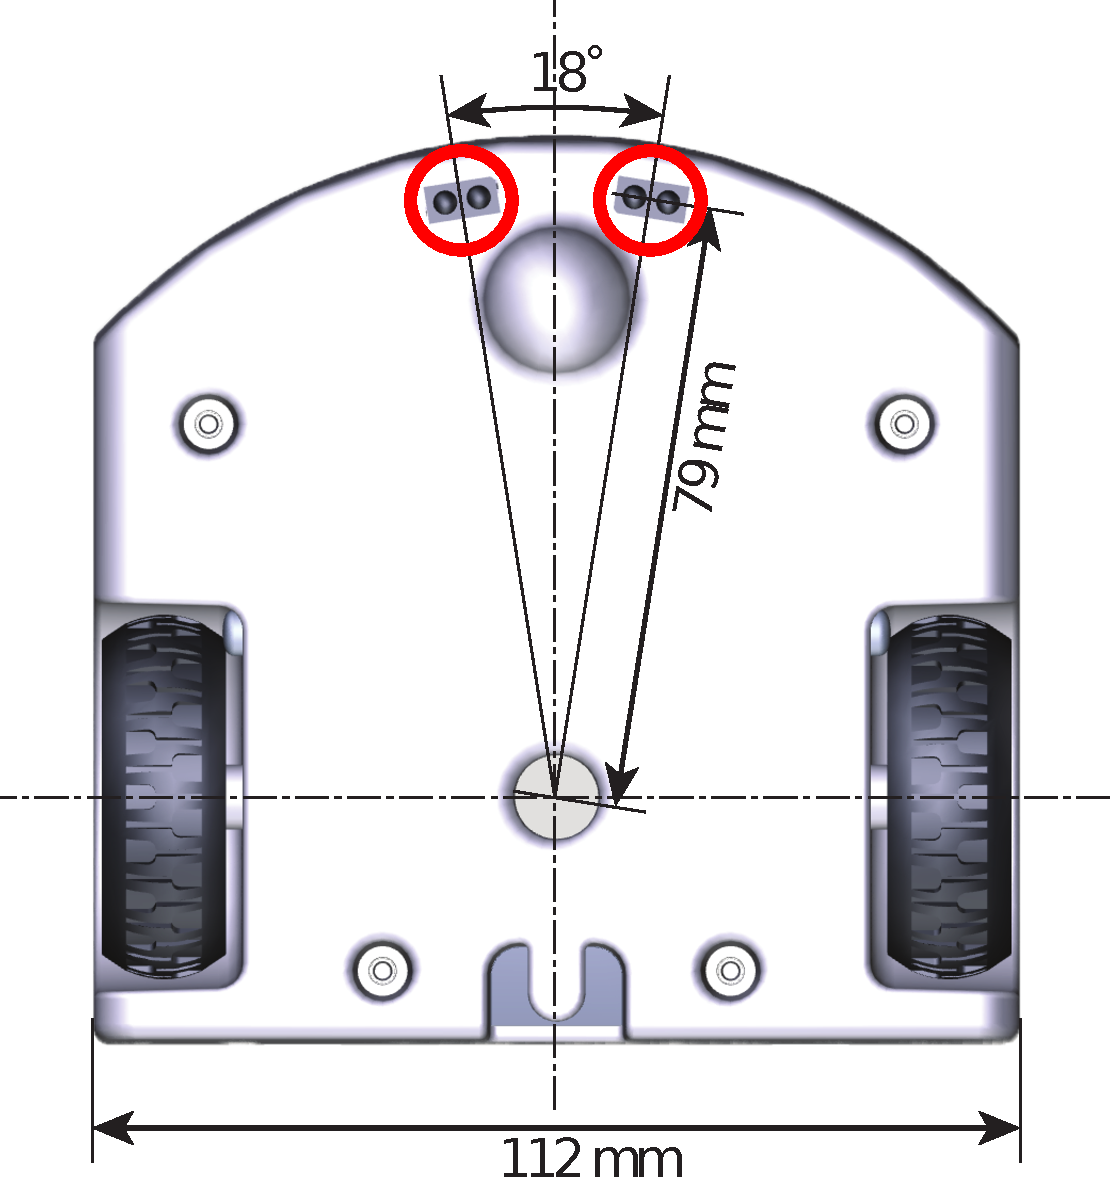
\includegraphics[width=.4\columnwidth]{thymio2-dimensions}
	
	\definecolor{inference}{named}{Blue}
	\definecolor{observation}{named}{Red}
	\definecolor{motion}{named}{Green}
	
	\begin{equation*}
	\textcolor{inference}{p(X_t|Z_{1:t},U_{1:t})} \propto \textcolor{observation}{p(Z_t | X_t)} \sum_{X_{t-1}} \textcolor{motion}{p(X_t|X_{t-1}, U_t)} \textcolor{inference}{p(X_{t-1} | Z_{1:t-1}, U_{1:t-1})}
	\end{equation*}
}

\frame
{
	\frametitle{Implementations}
	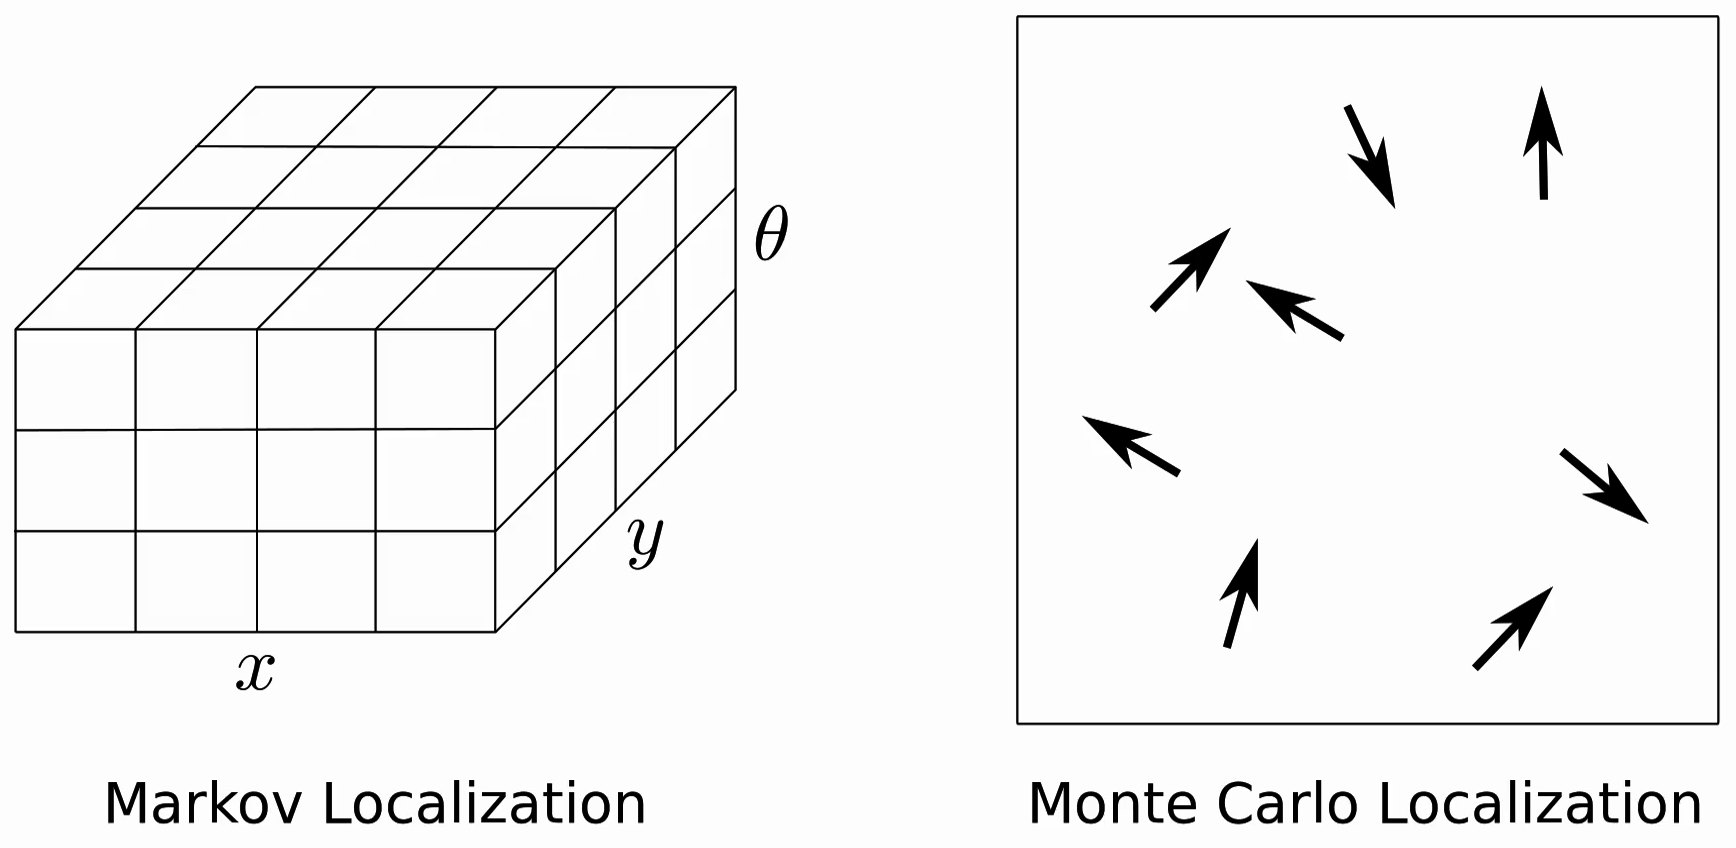
\includegraphics[width=\columnwidth]{implementations}
}

{
	\setbeamercolor{background canvas}{bg=black}
	\setbeamercolor{page number in head/foot}{fg=black}
	\frame
	{
		\begin{tikzpicture}[remember picture,overlay,shift=(current page.center)]
			\node at (0,0){
				\movie[width=\paperwidth]{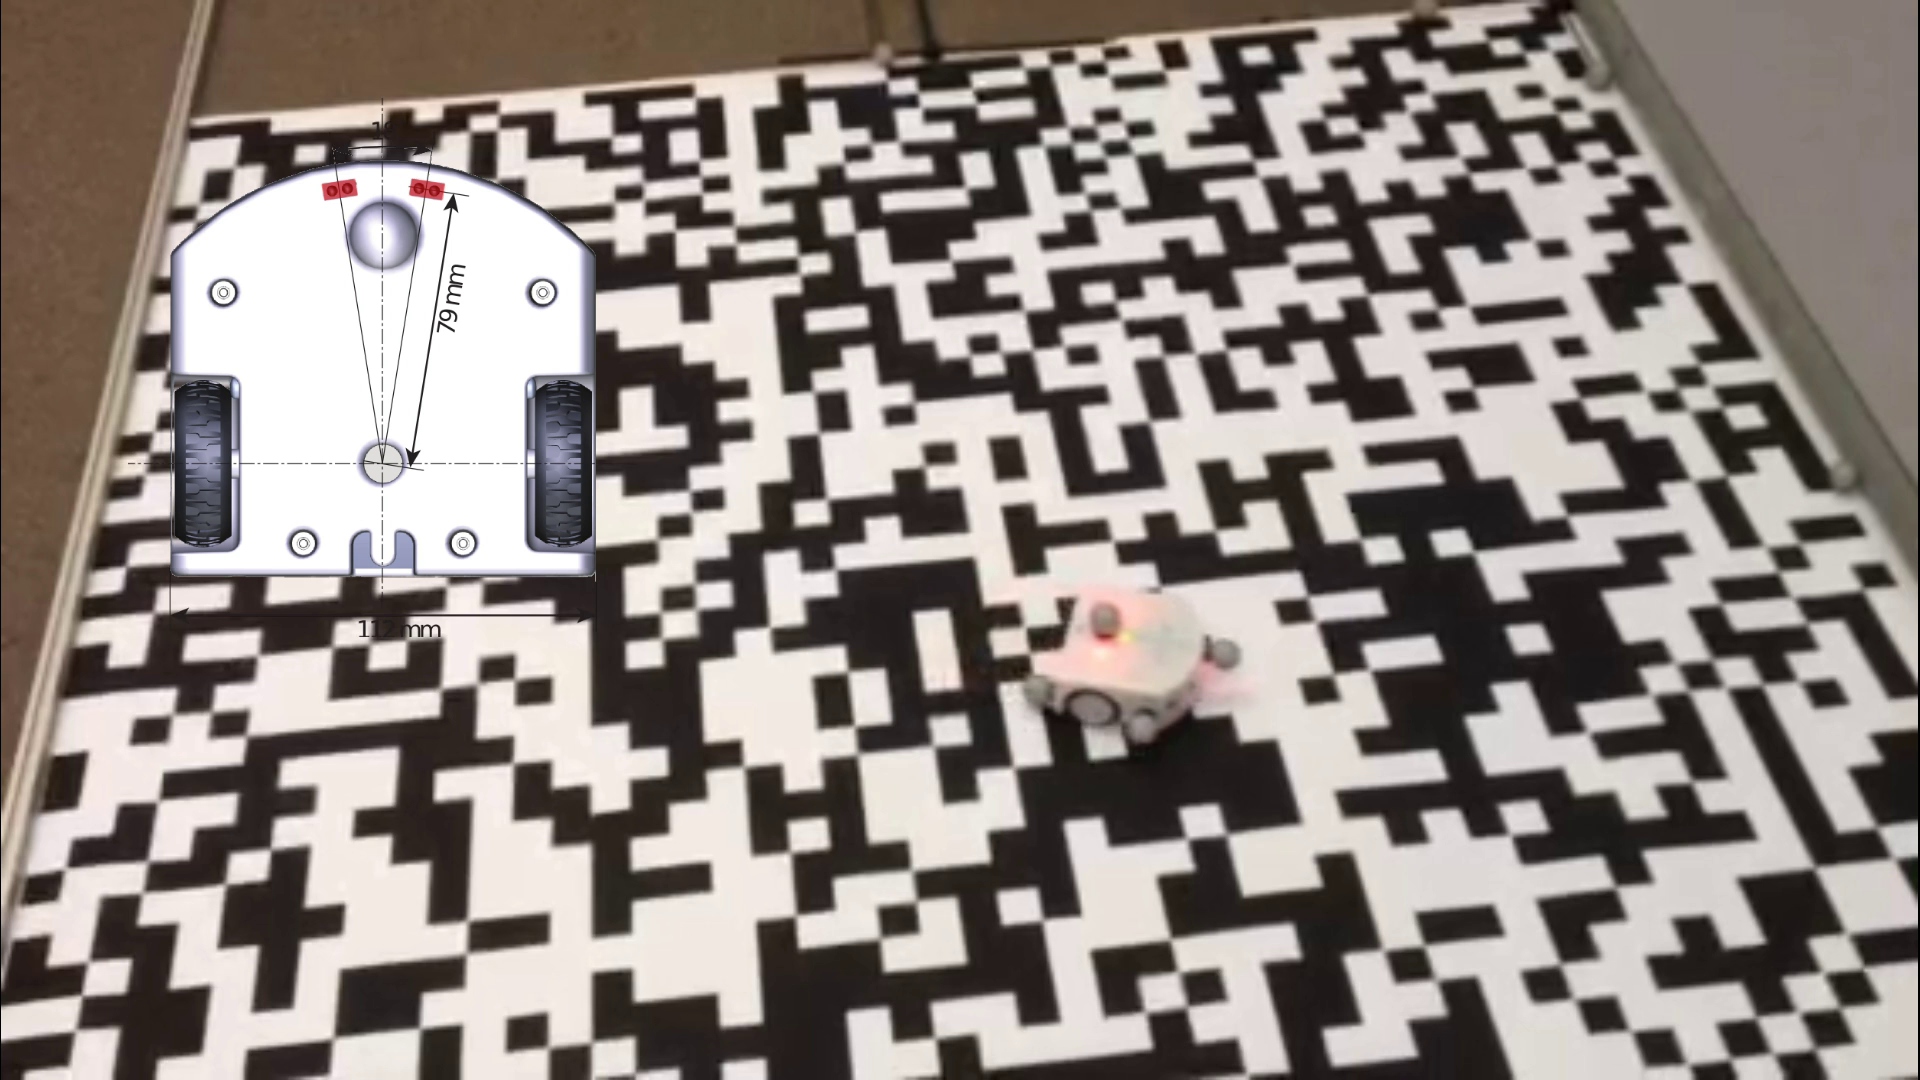
\includegraphics[width=\paperwidth]{data-acquisition}}{video/data-acquisition.mp4}
			};
		\end{tikzpicture}
	}
}

{
	\frame
	{
		\begin{tikzpicture}[remember picture,overlay,shift=(current page.center)]
			\node at (0,0){
				\movie[width=\paperwidth]{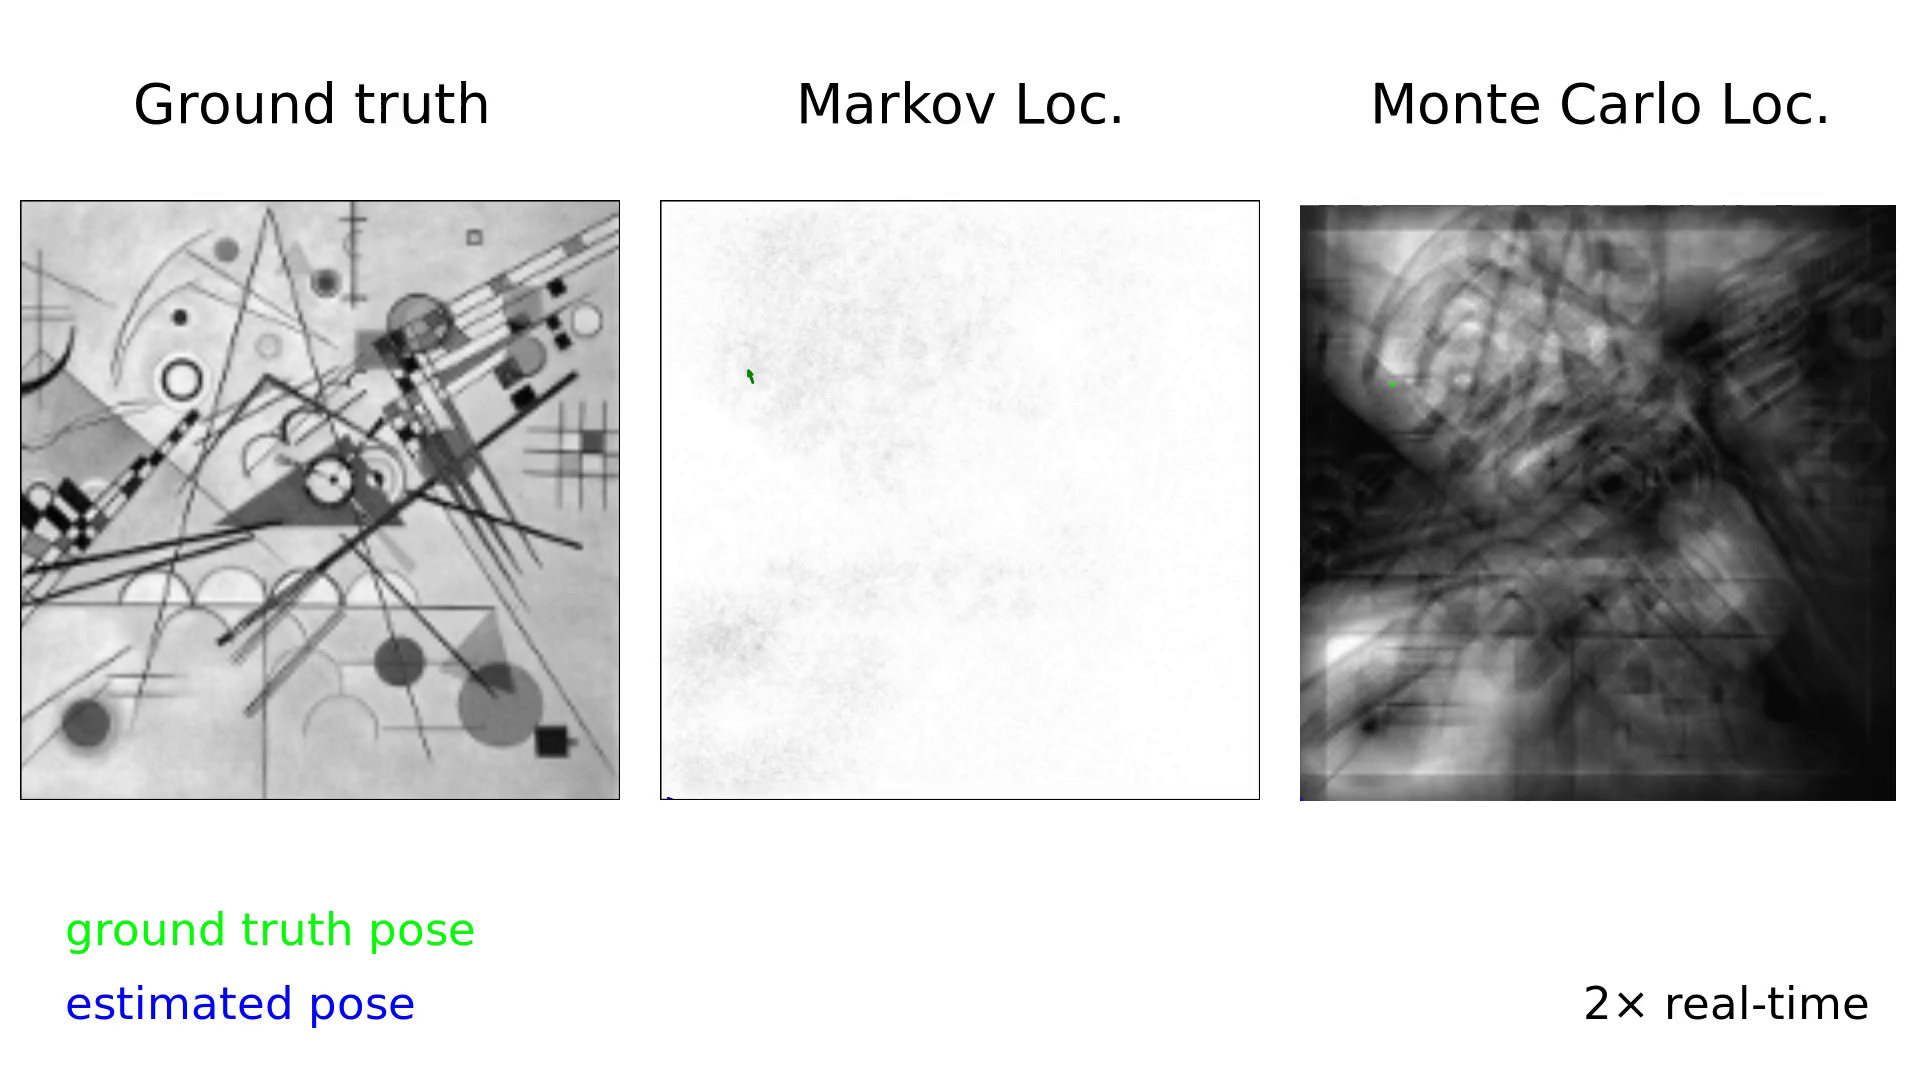
\includegraphics[width=\paperwidth]{prob-dists}}{video/prob-dists.mp4}
			};
		\end{tikzpicture}
	}
}


\frame
{
	\frametitle{Results – Basic localization}
	
	\makebox[.5\textwidth][c]{Markov Localization}\hfill
	\makebox[.5\textwidth][c]{Monte Carlo Localization}
	
	{\footnotesize
	\makebox[.5\textwidth][c]{\textcolor{gray}{varying number of discretization angles}}\hfill
	\makebox[.5\textwidth][c]{\textcolor{gray}{varying number of particles}}
	}
	
	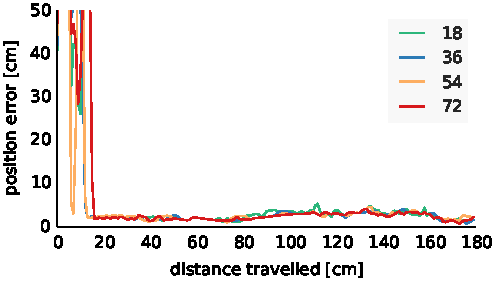
\includegraphics[width=.23\columnwidth]{ml-whole_random_2-xy}\hfill
	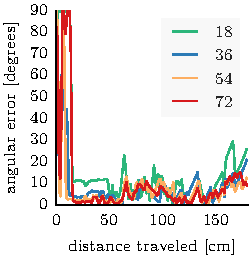
\includegraphics[width=.23\columnwidth]{ml-whole_random_2-theta}\hfill\hfill
	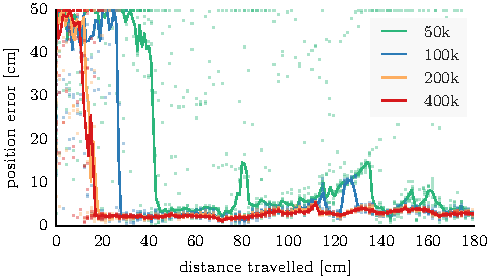
\includegraphics[width=.23\columnwidth]{mcl-whole_random_2-xy}\hfill
	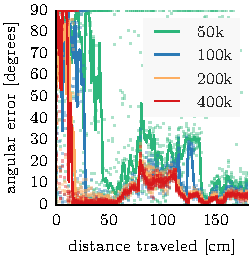
\includegraphics[width=.23\columnwidth]{mcl-whole_random_2-theta}
	
	\vspace{1em}

	\begin{itemize}
	\item Both methods eventually localize, precision depends on information acquisition
	\item Markov Localization: similar position error; angular error decreases until 54, then constant
	\item Monte Carlo Localization: many particles; error decreases until 200k, then constant
	\end{itemize}
}

\frame
{
	\frametitle{Results – Distance to converge}
	
	\makebox[.5\textwidth][c]{Markov Localization}\hfill
	\makebox[.5\textwidth][c]{Monte Carlo Localization}
	
	{\footnotesize
	\makebox[.5\textwidth][c]{\textcolor{gray}{varying number of discretization angles}}\hfill
	\makebox[.5\textwidth][c]{\textcolor{gray}{varying number of particles}}
	}
	
	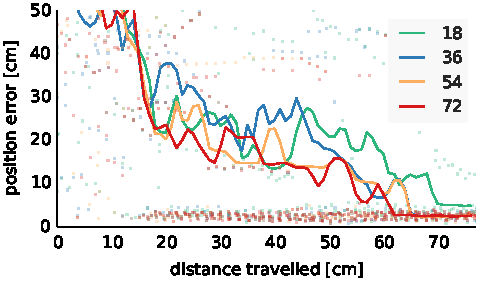
\includegraphics[width=.48\columnwidth]{ml-small_runs_random_12-xy}\hfill
	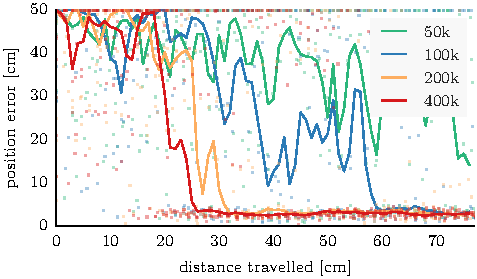
\includegraphics[width=.48\columnwidth]{mcl-small_runs_random_12-xy}

	\vspace{1em}

	\begin{itemize}
	\item Markov Localization: correct pose found after 20--25\,cm, excepted when robot turning on spot
	\item Monte Carlo Localization: with 400k, correct pose after 25\,cm, less particles increases distance
	\end{itemize}
}

\frame
{
	\frametitle{Results – Effect of ground map size}
	
	\makebox[\textwidth][c]{Markov Localization}
	
	{\footnotesize
	\makebox[\textwidth][c]{\textcolor{gray}{varying ground map size}}
	}
	
	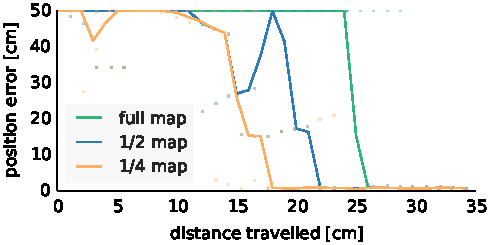
\includegraphics[width=.48\columnwidth]{ml-small_maps-xy}\hfill
	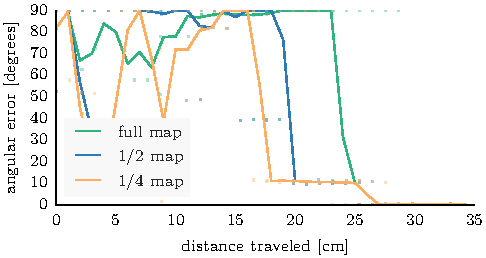
\includegraphics[width=.48\columnwidth]{ml-small_maps-theta}
	
	\vspace{1em}

	\begin{itemize}
	\item The smaller the map size, the shorter the distance to localize
	\item Theoretical estimation tool available in the paper
	\end{itemize}
}

\frame
{
	\frametitle{Results – Robot kidnapping}
	
	
	\makebox[.5\textwidth][c]{Markov Localization}\hfill
	\makebox[.5\textwidth][c]{Monte Carlo Localization}
	
	{\footnotesize
	\makebox[.5\textwidth][c]{\textcolor{gray}{varying number of discretization angles}}\hfill
	\makebox[.5\textwidth][c]{\textcolor{gray}{varying number of particles}}
	}
	
	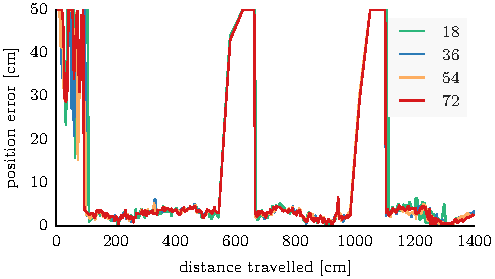
\includegraphics[width=.48\columnwidth]{ml-whole_random_long-xy} \hfill
	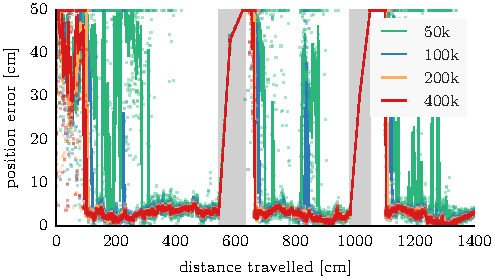
\includegraphics[width=.48\columnwidth]{mcl-whole_random_long-xy}
	
	\vspace{1em}

	\begin{itemize}
	\item Markov Localization: Robot relocalizes consistently after 100\,cm (5 times faster than prev. runs)
	\item Monte Carlo Localization: stable relocalization for 200k and more, unstable with 100k and less
	\end{itemize}
}

\frame
{
	\frametitle{Results – Robot kidnapping – confidence}
	
	
	\makebox[.5\textwidth][c]{Markov Localization}\hfill
	\makebox[.5\textwidth][c]{Monte Carlo Localization}
	
	{\footnotesize
	\makebox[.5\textwidth][c]{\textcolor{gray}{varying number of discretization angles}}\hfill
	\makebox[.5\textwidth][c]{\textcolor{gray}{varying number of particles}}
	}
	
	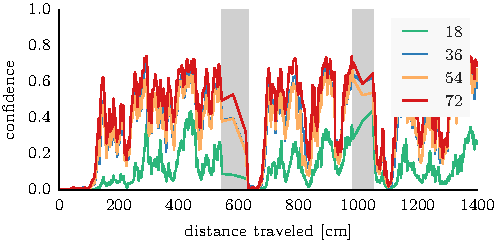
\includegraphics[width=.48\columnwidth]{ml-whole_random_long-conf} \hfill
	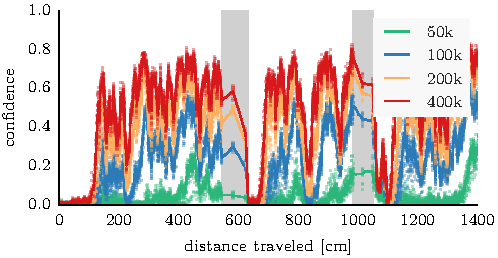
\includegraphics[width=.48\columnwidth]{mcl-whole_random_long-conf}
	
	\vspace{1em}

	\begin{itemize}
	\item Self-confidence measure: ratio of probability mass around maximum
	\item High confidence indicates a peaked probability distribution
	\item Effective to detect kidnapping
	\end{itemize}
}

\frame
{
	\frametitle{Results – Computational cost}
	
	\begin{center}
	{\small \textcolor{gray}{150$\times$150 cm ground pattern, Lenovo laptop T450s, Intel Core i7 5600U, 2.6\,GHz}}
	
	\vspace{.5em}
	
	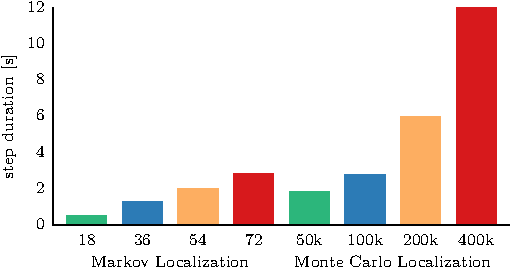
\includegraphics[width=.65\columnwidth]{cpu_load}
	\end{center}
	
	\begin{itemize}
	\item Markov Localization: linear cost
	\item Monte Carlo Localization: amortized linear cost
	\end{itemize}
}

\frame
{
	\frametitle{Results – Real-time localization}
	
	{\footnotesize
	\makebox[\textwidth][c]{\textcolor{gray}{Markov Localisation, 36 discretization angles, A2}}
	}

	\makebox[.15\textwidth][c]{Breugel}\hfill
	\makebox[.15\textwidth][c]{Van Gogh}\hfill
	\makebox[.15\textwidth][c]{Kandinsky}\hfill
	\makebox[.15\textwidth][c]{Vermeer}\hfill
	\makebox[.15\textwidth][c]{Babar}\hfill
	\makebox[.15\textwidth][c]{Child's drawing}

	\vspace{.6em}

	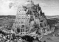
\includegraphics[width=.15\textwidth,interpolate=false]{maps/breugel_babel_A2} \hfill
	
\includegraphics[width=.15\textwidth,interpolate=false]{maps/van-gogh_starry-night_A2} \hfill
	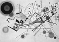
\includegraphics[width=.15\textwidth,interpolate=false]{maps/kandinsky_comp-8_A2} \hfill
	
\includegraphics[width=.15\textwidth,interpolate=false]{maps/vermeer_girl-pearl_A2} \hfill
	
\includegraphics[width=.15\textwidth,interpolate=false]{maps/babar_A2} \hfill
	
\includegraphics[width=.15\textwidth,interpolate=false]{maps/child-drawing_tooth-fairy_A2}

	\vspace{.7em}

	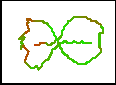
\includegraphics[width=.15\textwidth]{breugel_babel-traj} \hfill
	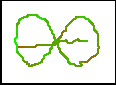
\includegraphics[width=.15\textwidth]{van-gogh_starry-night-traj} \hfill
	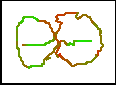
\includegraphics[width=.15\textwidth]{kandinsky_comp-8-traj} \hfill
	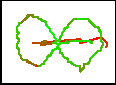
\includegraphics[width=.15\textwidth]{vermeer_girl-pearl-traj} \hfill
	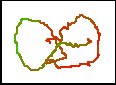
\includegraphics[width=.15\textwidth]{babar-traj} \hfill
	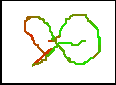
\includegraphics[width=.15\textwidth]{child-drawing_tooth-fairy-traj}

	\vspace{.7em}

	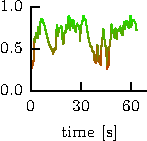
\includegraphics[width=.15\textwidth]{breugel_babel-conf} \hfill
	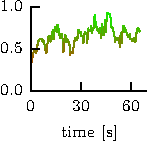
\includegraphics[width=.15\textwidth]{van-gogh_starry-night-conf} \hfill
	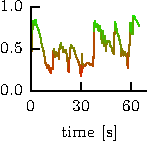
\includegraphics[width=.15\textwidth]{kandinsky_comp-8-conf} \hfill
	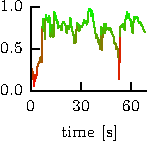
\includegraphics[width=.15\textwidth]{vermeer_girl-pearl-conf} \hfill
	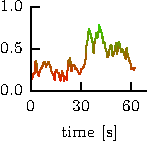
\includegraphics[width=.15\textwidth]{babar-conf} \hfill
	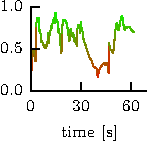
\includegraphics[width=.15\textwidth]{child-drawing_tooth-fairy-conf}
}

\frame
{
	\frametitle{Outlook and conclusion}

	\begin{itemize}
	\item Inexpensive robots with low-bandwidth sensors can perform absolute localization
	\item Ground visual pattern and inexpensive infrared sensors fits collective robotics
	\item Significant processing needs, but \textsc{gpu} implementation would bring it to embedded systems
	\item Can be used as an educational tool to teach Bayesian localization
	\end{itemize}
	
	\vspace{.5em}
	
	\hspace{2em}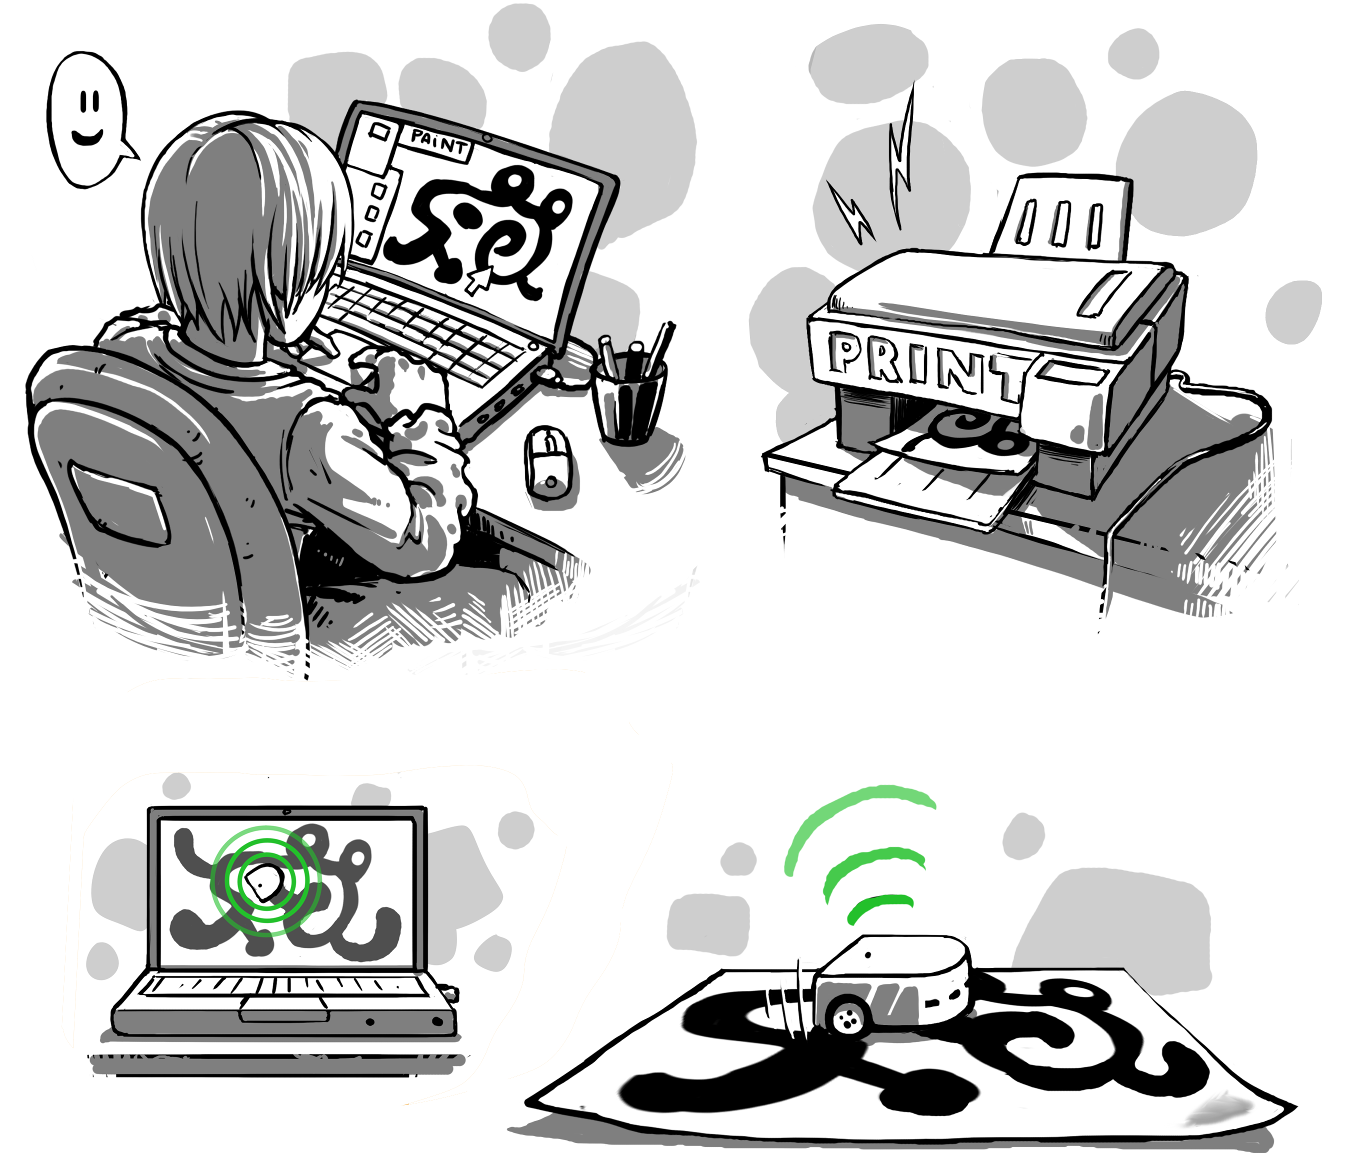
\includegraphics[width=.4\columnwidth]{process_creation_col_small}
	\hfill
	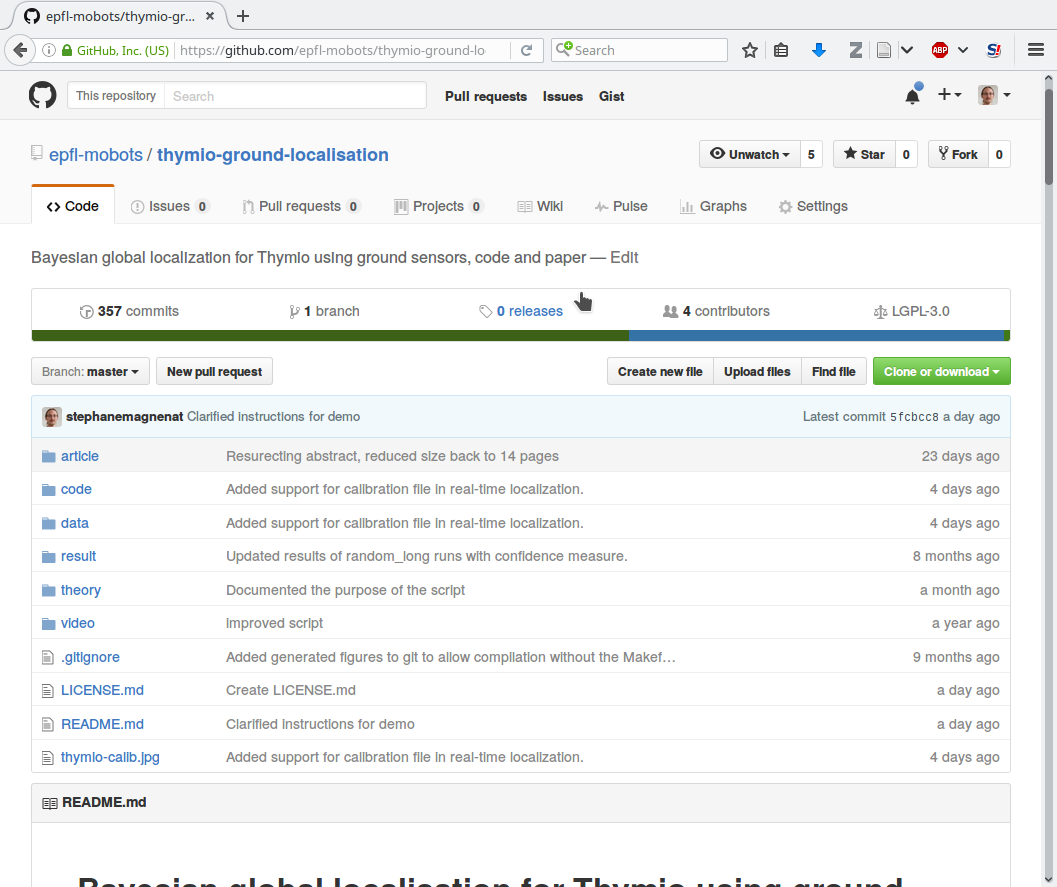
\includegraphics[width=.4\columnwidth]{github-page}\hspace{2em}
}

\frame
{
	\begin{tikzpicture}[remember picture,overlay,shift=(current page.center)]
		\node at (0,.5){
			{\Large \sourcesanspro Thank you for your attention.}
		};
		\node at (0,-.5){
			{\url{https://github.com/epfl-mobots/thymio-ground-localisation}}
		};
	\end{tikzpicture}
}



\end{document}
